\section{Miscellaneous}

\subsection{Field Construction}
\begin{figure}[b!]
\centering
\centerline{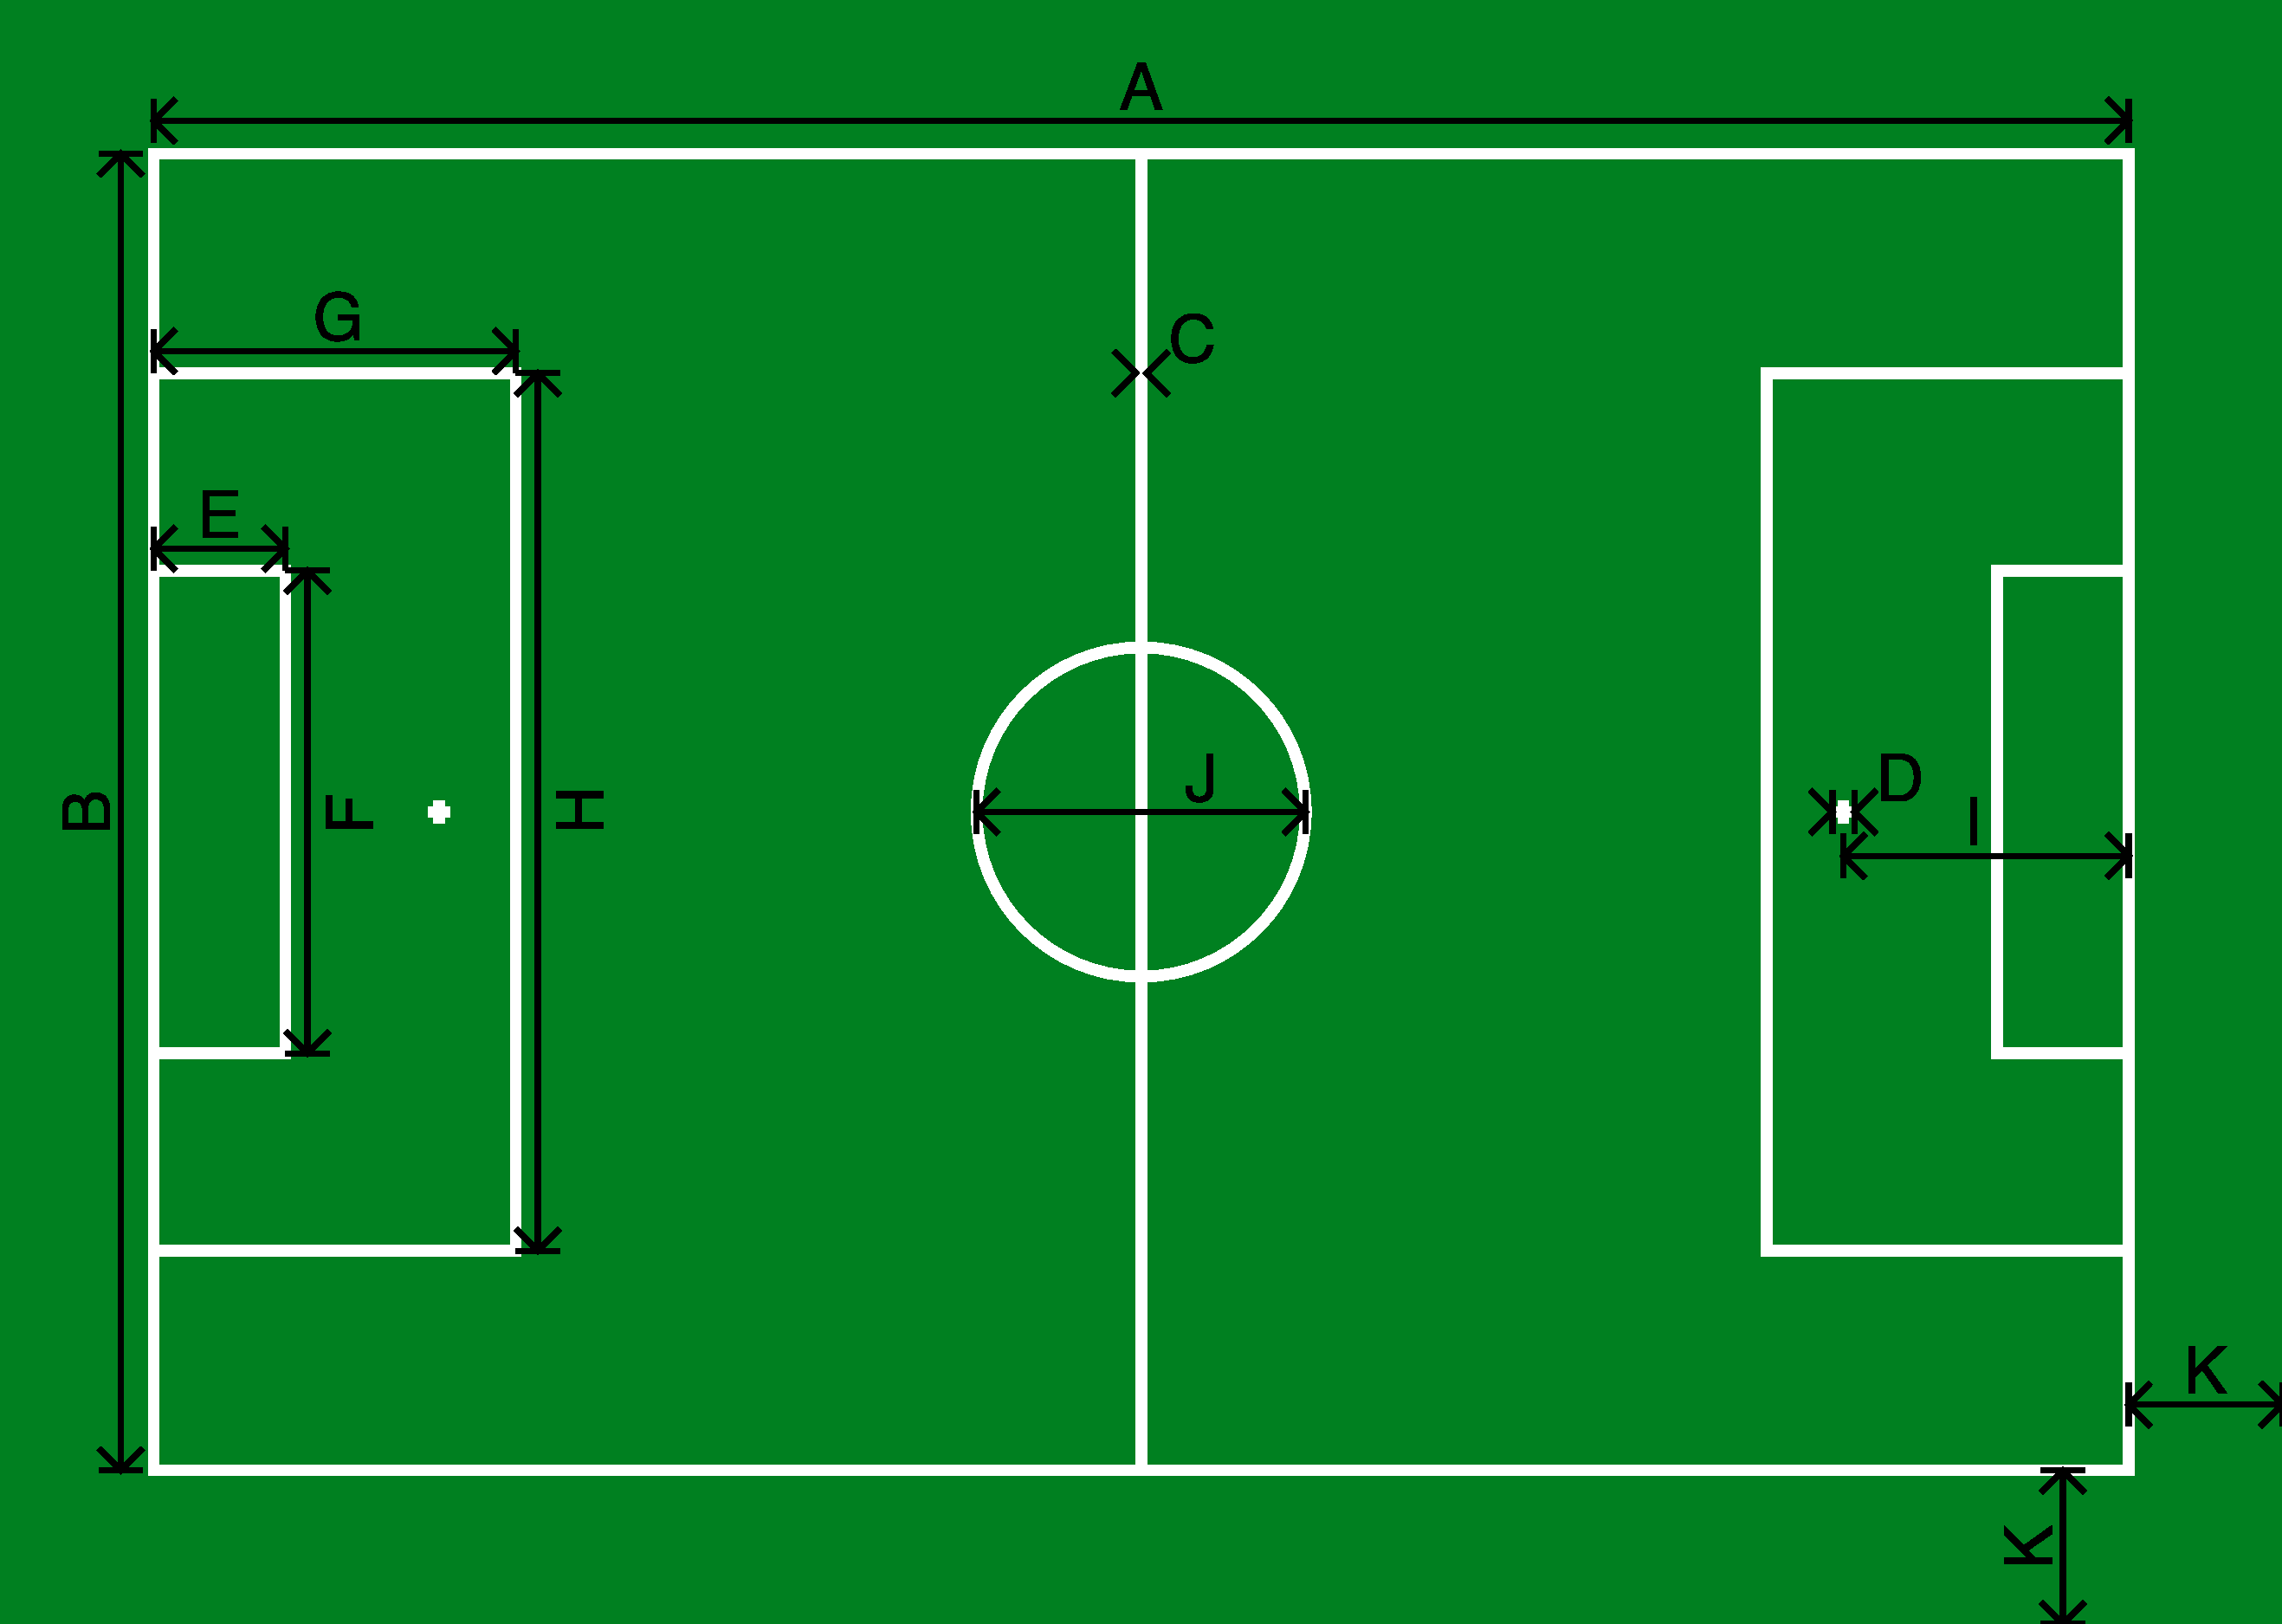
\includegraphics[width=\columnwidth]{figs/fieldDimensions2020.pdf}}
\vspace{1ex}
\begin{tabular}{| l | l | l |}
ID & Description & Length (in mm) \\
\hline \hline
A & Field length & 9000 \\
\hline
B & Field width & 6000 \\
\hline
C & Line width & 50 \\
\hline
D & Penalty cross size & 100 \\
\hline
E & Goalbox area length & 600 \\
\hline
F & Goalbox area width & 2200 \\
\end{tabular}
\begin{tabular}{|l|l|l|}
ID & Description & Length (in mm) \\
\hline \hline
G & Penalty area length & 1650* \\
\hline
H & Penalty area width & 4000* \\
\hline
I & Penalty cross distance & 1300 (1400*) \\
\hline
J & Center circle diameter & 1500 \\
\hline
K & Border strip width & 700 \\
\hline
 &  &  \\
\end{tabular}
\caption{Schematic diagram of the soccer field (not to scale) and corresponding dimensions in mm.  Note that measurements on this diagram are made to the center of lines.}
\label{fig:field_construction}
\end{figure}
